%% Base on http://tex.stackexchange.com/questions/150900/latex-coding-for-statement-of-purpose

\documentclass{article}
\usepackage[
  a4paper,
  margin=1in,
  headsep=4pt, % separation between header rule and text
]{geometry}
\usepackage[dvipsnames]{xcolor}
\usepackage{graphicx} 
\usepackage{fancyhdr}
\usepackage{tgschola}
\usepackage{lastpage}
\usepackage[numbers,sort&compress]{natbib}
\bibliographystyle{ksfh_nat}
\usepackage{xcolor}
\usepackage{sectsty}
\chapterfont{\color{blue}}  % sets colour of chapters
\sectionfont{\color{cyan}}
\subsectionfont{\color{darkgray}}
\subsubsectionfont{\color{gray}}
\usepackage[T1]{fontenc}
\usepackage[utf8]{inputenc}
\usepackage{lmodern}
\pagestyle{fancy}
\fancyhf{}
\fancyhead[C]{%
  \footnotesize\sffamily
  \yourname\quad
  web: \textcolor{blue}{\itshape\yourweb}\quad
  \textcolor{blue}{\youremail}}
\fancyfoot[C]{Page \thepage\ of \pageref{LastPage}}

\newcommand{\soptitle}{\textbf{Magnetic filaments: State of the art}}

\newcommand{\yourname}{Deniz Mostarac, MSc}
\newcommand{\youremail}{email@address.edu}
\newcommand{\yourweb}{https://www.abcd.com/}

\newcommand{\statement}[1]{\par\medskip
  \textcolor{blue}{\textbf{#1:}}\space
}

\usepackage[
  breaklinks,
  pdftitle={\yourname - \soptitle},
  pdfauthor={\yourname},
  unicode
]{hyperref}

\begin{document}

\begin{center}\LARGE\soptitle\\
\large application for Uni:Docs by \yourname\ (PhD student in Diopolar Soft Matter group of Universiy in Vienna)
\end{center}

\textcolor{NavyBlue}{\hrule height 2pt}
\vspace{1pt}
\textcolor{NavyBlue}{\hrule height 4pt}


\section[colour=blue]{Current state of research and own research goals}
\subsection{Current state of research}
Polymer stimuli-responsive materials are one of the central research topics in modern soft mater physics \cite{balazs2006nanoparticle,hu2010responsive}. Currently available responsive materials are sensitive to a broad range of stimuli, like temperature and electromagnetic radiations,\cite{jochum2013temperature} pH,\cite{dai2008ph} ionic strength,\cite{magnusson2008ion} specific additives and substances,\cite{ulijn2006enzyme} or external fields.\cite{roy2011biological}. However, most of such materials are toxic of deadly to living cells and organisms. The nonexistence of known polymer substances with pronounced magnetic properties (magnetic fields of only a couple mT have shown not to interfere with any known bio-processes known), except for a few compounds at very low temperatures,\cite{rajca2001magnetic,kamachi2002magnetic,blundell2004organic} suggests the possible necessity of combination of polymers with magnetic micro- or nanoparticles.\cite{thevenot2013magnetic}\\\\
Ferrofluids and magneto-rheological fluids are usually created by adding independent micron or sub-micron sized magnetic particles to a carrier fluid to form a colloidal suspension. These magnetic systems have been studied theoretically and experimentally for more than forty years.\cite{holm2005structure,sanchez2015effect,de2011magnetorheological} Numerous systems based the self-assembly mechanism have been studied in recent years, such as patchy colloids,\cite{bianchi2011inverse,preisler2014equilibrium,smallenburg2014erasing} blunt-end DNA duplexes,\cite{nakata2007end,zanchetta2010right,kantorovich2013calculate,rovigatti2014gels} and magneto-rheological suspensions,\cite{shulman1986structure,park2010magnetorheology} as self-assembly has been recognised as a key mechanism for appropriating soft mater systems as building blocks of enhanced magnetic fluids and complex magneto-responsive structures. Such self-assembled structures can further be stabilized and/or modified by introducing additional bonding mechanisms, such as crosslinking, to the system. This allows the creation of supra-molecular structures with specific properties, such as magnetic gels \cite{frank1993voltage,zrinyi1998kinetics,Weeber_2012} and DNA origami structures.\cite{Rothemund_2006,Pal_2010,Zadegan_2012} \\\\
Using pre-crosslinked structures in place of plain nanoparticles has a significant impact on the equilibrium and assembly properties. Most existing cross-linking procedures for synthesis of such composite materials are based on the functionalization of the nanoparticle surface. Interesting examples of such realized systems are the field-induced assembly of polymer-coated magnetic particles into dense arrays of non-permanent linear chains, adopting a transient polymer brush-like structure on a surface,\cite{Tokarev_2014} or the direct embedding of magnetic nanoparticles into actual polymer brushes.\cite{Choi_2008} Permanent chains of polymer crosslinked magnetic particles, were in fact synthesized for the first time more than one decade ago with the purpose to work as magnetically driven microfluidic propellers.\cite{Dreyfus_2005}\\\\ In recent years, such magnetic chains have found a growing range of applications.\cite{WANG_2011} Semi-flexible fiber structures of magnetic nanoparticles have been obtained instead by crosslinking them in bunches.\cite{Bharti_2015} Chain-like aggregates of MP’s have been shown as promising candidates for the design of recording media and sensor systems, biomedical materials and tuneable photonic crystals.\cite{wang2011magnetic} Initial need for synthesis of MF systems arose for magnetically controlled microfluidic implementations. In particular, the main application explored to date, is their use as magnetically actuated artificial cilia, which can be used to create micro-swimmers for future,\cite{dreyfus2005microscopic,cebers2005flexible,belovs2009erratum,javaitis2011physics} externally controlled drug delivery devices.\cite{peyer2013bio} It is also possible to create magnetically actuated microfluidic pumpers and mixers,\cite{singh2005synthesis,evans2007magnetically,babataheri2011tethered} a function essential for lab-on-chip devices and other microfluidic systems. Some investigations have been made into MF implementations as micro-mechanical sensors,\cite{goubault2003flexible} as well as in the context of contrast agents for magnetic resonance measurements. Here, they have great potential, due their higher sensitivity to magnetic fields,\cite{corr2008linear} compared to currently used agents. More generally, MFs are promising candidates to replace conventional magnetic fluids,\cite{2013,de2011magnetorheological} in any application that may benefit form the enchantment of magnetorheological responsiveness. MF use can make design of magnetically controlled microfluidic valves and micro-filter devices significantly simpler.\cite{doyle2002self} In fact, increased magnetorheological responsiveness might find uses for magnetically controlled dampeners or polishing systems.\cite{2013,de2011magnetorheological,park2010magnetorheology}
\newpage
\textcolor{NavyBlue}{\hrule height 2pt}
\vspace{1pt}
\textcolor{NavyBlue}{\hrule height 4pt}
\subsection{Positioning of own research project}
Within the broad spectrum of stimuli one could use to modify material properties, responsiveness to electric and magnetic fields proves to be of extraordinary potential.\cite{roy2011biological} This is due to the highly dynamic control of the intensity and the spatial resolution of the stimulus, one can achieve. Polymers with a significant magnetic response are rare and exhibit such properties only for a specific temperature range.\cite{rajca2001magnetic,Kamachi_2002,blundell2004organic} \textbf{Our approach for the construction of smart materials with sophisticated magnetic response by embedment of magnetic micro- or nanoparticles (MP’s) within permanently cross-linked structures (i.e. brush structures), such as polymer arrays or networks, is the cutting edge of such research, with great potential for technological applications.} Cross-linked structures have immediate advantages over other magneto-fluids class materials.\cite{2013,de2011magnetorheological} Cross-linking allows for higher structural integrity of the system (i.e higher resistance to shear stress under flow), which results in stabilisation of the aggregates, in addition to the increased tunability of the system. \textbf{Most existing cross-linking procedures for synthesis of such composite materials are based on the functionalization of the MP’s surface. However, they provide limited control over the material structure.} \\\\
In particular, the distribution of MP’s within a polymer network, cannot be finely tuned. This limits the responsiveness of the magnetic system. \textbf{Despite the vast potential for application, most of the technological implementation examples we mention, remain either unrealised, or lack further theoretical and experimental investigations.} One-dimensional cross-linking of ferromagnetic nanoparticles has only been achieved in terms of rigid filaments, which imposes extreme limitations on potential applications.\cite{zhou2008coating,xiong2007formation,zhang2008fabrication,ma2012fabrication} The end product should be a permanent, semi-flexible chain with magneto-responsive properties. These systems, known as magnetic filaments (MFs), are the main research subject of our project. \textbf{We aim to, in close collaboration with our international partner, computationaly and analytically investigate, synthesise and characterise fully flexible, structurally malleable MF’s and Supramolecular magnetic filament brushes, based on programmable DNA-nanoparticle assembly.}\cite{Maye_2009, Sun_2012, Sun_2013, Zhang_2013, Tian_2015}. The principal aim of this novel technique is to manipulate the self assembly of NP’s by creating hybrid complexes of DNA origami frames and nanoparticles, with anisotropic and selective bonding properties, allowing for unheard of control of the microstructure and magnetic response of the final MF based superstructures, where we refer to supramolecular magnetic filment brushes.

\section{Goals and work plan}
\subsection{Scientific goal of the dissertation}
\textbf{Our project aims to fill the gaps in both synthesis and fundamental understanding of MFs, in order to pave way for the development of improved magneto-responsive materials and new applications.} During my stay at Columbia University, in the group of Prof. Gang, we will push forward a novel synthesis technique, that will provide a higher degree of control of the properties of MFs. This would, for the first time, enable synthesis of one-dimensional chains of cross-linked nanoparticles.  We will identify and investigate the characteristics of these system that make them promising building blocks of complex, nanostructured magnetic materials and magnetic fluids with improved properties. \textbf{By combining experiments (Gang group), theory and computer simulation (Kantorovich group), we want to pioneer development of such systems.} Our approach should overcome the limitations of currently available methods, reduce the difficulty of synthesis for surface grafted systems while yielding MFs with significant flexibility of the filament backbone.
\textbf{The main appeal of MFs, in technological applications, stems from their ability to react to an externally applied magnetic field.} The way a MF responds to an applied field depends on multiple factors, such as nanoparticle size, material, temperature, number of magnetic particles in the structure and flexibility and length of the cross-linkers. Provided a reliable computational model, characterisation and determination of the optimal properties of MFs, truncates to a simple parameter change within the model. This saves a significant amount of money and time one would otherwise need in a real experiment. In fact, the savings are so significant, that many applications would otherwise simply not be feasible. \textbf{Therefore, in the first phase of our research, prior to synthesis, extensive molecular dynamics simulations will be performed. In this way, the influence of each of the aforementioned factors will be studied in detail and precisely determined.}
The second phase of our research is concerned with synthesis, support and characterisation of the physical properties of magnetic filament samples, using a novel experimental technique. \textbf{Successful realisation of this phase requires a plethora of manpower, experimental (Gang group) and theoretical  (Kantorovich Group) expertise, interdisciplinary research and flexibility, along with sophisticated and expensive equipment one needs for synthesis of MFs.} We feel that the Marshall scholarship is a necessary step toward our goals, as such cooperation can only be realised at Columbia University, with me being a guest in Prof. Gangs Group. This would be of great personal value, as this unique, multidisciplinary learning and training opportunity puts me in a great position career-wise. \textbf{We plan to, in close collaboration with our experimental partners, provide a theoretical and computational modelling background to the synthesis, provide desired physical properties, based on our previous studies of MF systems and refine our theoretical models according to the new information.}

\subsection{Work Plan}
\subsubsection{Phase 1}
Realisation of our research plan is based on a well coordinated and purposefully directed effort form both  the Kantorovich and the Gang group. Research phases, as presented bellow, are constructed as such, so that the work done by both sides, separately at first, supplements each other, prepares an efficient framework, to maximise the productivity of my stay in Columbia. In this way, a conjoint, concentrated effort will result in successful synthesis and experimental characterisation of MFs, as well as permit fine-tuning of our computer simulation models. We are confident we can uphold the schedule we propose here, and justify these expectations with the following:
\begin{itemize}
    \item{\textcolor{cyan}{Kantorovich group}, of which I am a part of, has a world recognised expertise in computer simulations of magnetic soft matter and was the first group to propose simulation approaches of MFs.}
    \item{\textcolor{MidnightBlue}{Gang group’s} work, represents the cutting edge of modern physical chemistry and, to the best of our knowledge, holds a worldwide, leading position in nanoscopic design.}
\end{itemize}
\begin{figure}[h]
\centering
  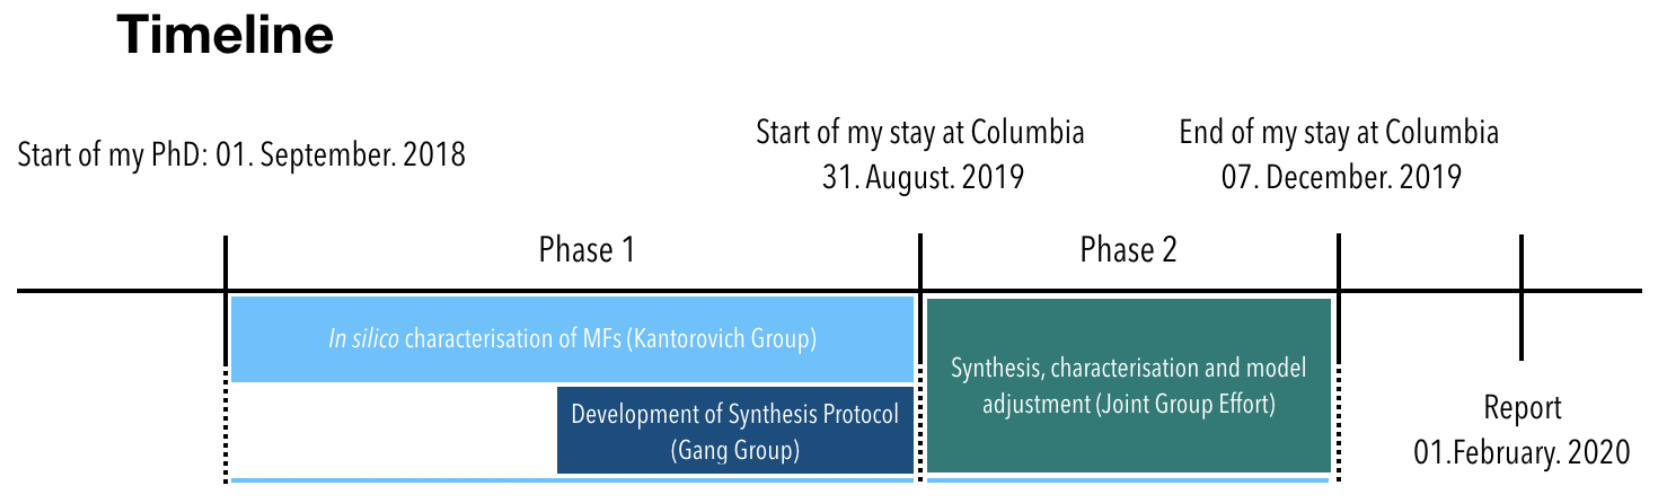
\includegraphics[height=4cm]{fig1}
\end{figure}
If granted, the Marshall Scholarship puts me in the position to connect the two groups, gives me the opportunity to obtain unique training in state of the art experimental and computational techniques and opens the possibility, for me to contribute to implementation of MFs in novel technological applications.
\begin{itemize}
    \item{\textbf{\textcolor{cyan}{Task 1 (September-November 2018)}}: development and implementation of a computational model of MFs with super-paramagnetic particles, recognising that each particle not only feels an applied field, but also the field created by other MPs in the system. All previous models treated magnetic particles exclusively as permanently magnetised.}
    \item{\textbf{\textcolor{cyan}{Task 2 (November. 2018-January 2019)}}: extensive computer simulations of a single MF, varying the following parameters: 
    \begin{itemize}
        \item{the value of particle saturation magnetisation (equivalent to changing the size and/or the particle material in the experiment) }
        \item{the equilibrium length of the spring, connecting the particles (equivalent to changing the DNA cages size in the experiment, see below)}
        \item{filament rigidity (to vary the length of the connecting DNA strands in the experiment, see below)}
        \item{filament length and magnetic particle positioning within MFs — all particles can be magnetic, every other particle can be magnetic, etc., (representing the number of connected cages and their occupancy by nanoparticles, see below). The simulations should be performed at different values of an applied magnetic field. Reliable statistics will be accumulated.}
    \end{itemize}
    }
    \item{\textbf{\textcolor{cyan}{Task 3 (January-March 2019)}}: analysis of MF magnetisation curves and end-to-end distance as a function of applied magnetic field. Analysis should be performed for all studied systems, and its results will be compared with corresponding properties of MFs with permanently magnetised particles. The most promising (the most magnetically responsive) MF candidates will be determined and communicated to the Gang group.}
    \item{\textbf{\textcolor{cyan}{Task 4 (March-May 2019)}}: development and implementation of the computational model of suspensions of MFs. Special attention is given to the behaviour of the MFs under flow of the background fluid. We will effort in code optimisation, as computing performance starts to be a factor (systems become orders of magnitude larger than the ones studied in Tasks 1-3). }
    \item{\textbf{\textcolor{MidnightBlue}{Task 1 (March-May 2019)}}: verification of the feasibility of synthesis for candidates, as determined by us. If the candidates proposed by our theoretical considerations are experimentally not realistic options, the optimal configurations would be reassessed via an active data exchange between the groups. By the end of this period, a set of MF candidates will be chosen.}
    \item{\textbf{\textcolor{MidnightBlue}{Task 2 (June-August 2019)}}:  implementation of the synthesis protocol for the types of filaments, as previously agreed in \textcolor{cyan}{Task 3}}
\end{itemize}
\subsubsection{Phase 2}
\begin{itemize}
    \item{\textbf{\textcolor{PineGreen}{Task 1 (September 2019)}}: synthesis of MFs according to the specifications agreed in Tasks 3 of Phase 1, with various chain lengths. Synthesis monitoring and characterisation using TEM microscopy (no magnetic field) will be performed, along with end to end distance analysis. We will arrange the possibility to do in field measurements. }
    \item{\textbf{\textcolor{PineGreen}{Task 2 (October 2019)}}: adjustment of the simulation protocol, to match the experimental systems as close as possible, along with SAXS and AFM measurement based characterisation. Applied field amplitudes are to be selected based on the new simulation protocol.}
    \item{\textbf{\textcolor{PineGreen}{Task 3 (November 2019)}}: extensive analysis of the data from both simulations and experiments. Preparation for larger-scale (suspensions) experiments, along with classification of available and studied MFs according to their magnetic and mechanical properties will be performed.}
\end{itemize}
\subsection{Description of methods}
\subsubsection{Phase 1}
\begin{itemize}
    \item{\textbf{\textcolor{cyan}{Tasks 1–3}}: Coarse grained Molecular dynamics simulations in ESPReSso software simulation package.\cite{limbach2006espresso} A single filament is represented as a set of spheres, connected by springs (Fig. 1). Super-paramagnetism of particles is taken into account through an iterative procedure, where we reassign the values and the orientations of particles magnetic dipole moments, depending on the total magnetic field in the centre of particles mass, using a Langevin function, to allow for non-linear effects.}
\begin{figure}[h!]
\centering
  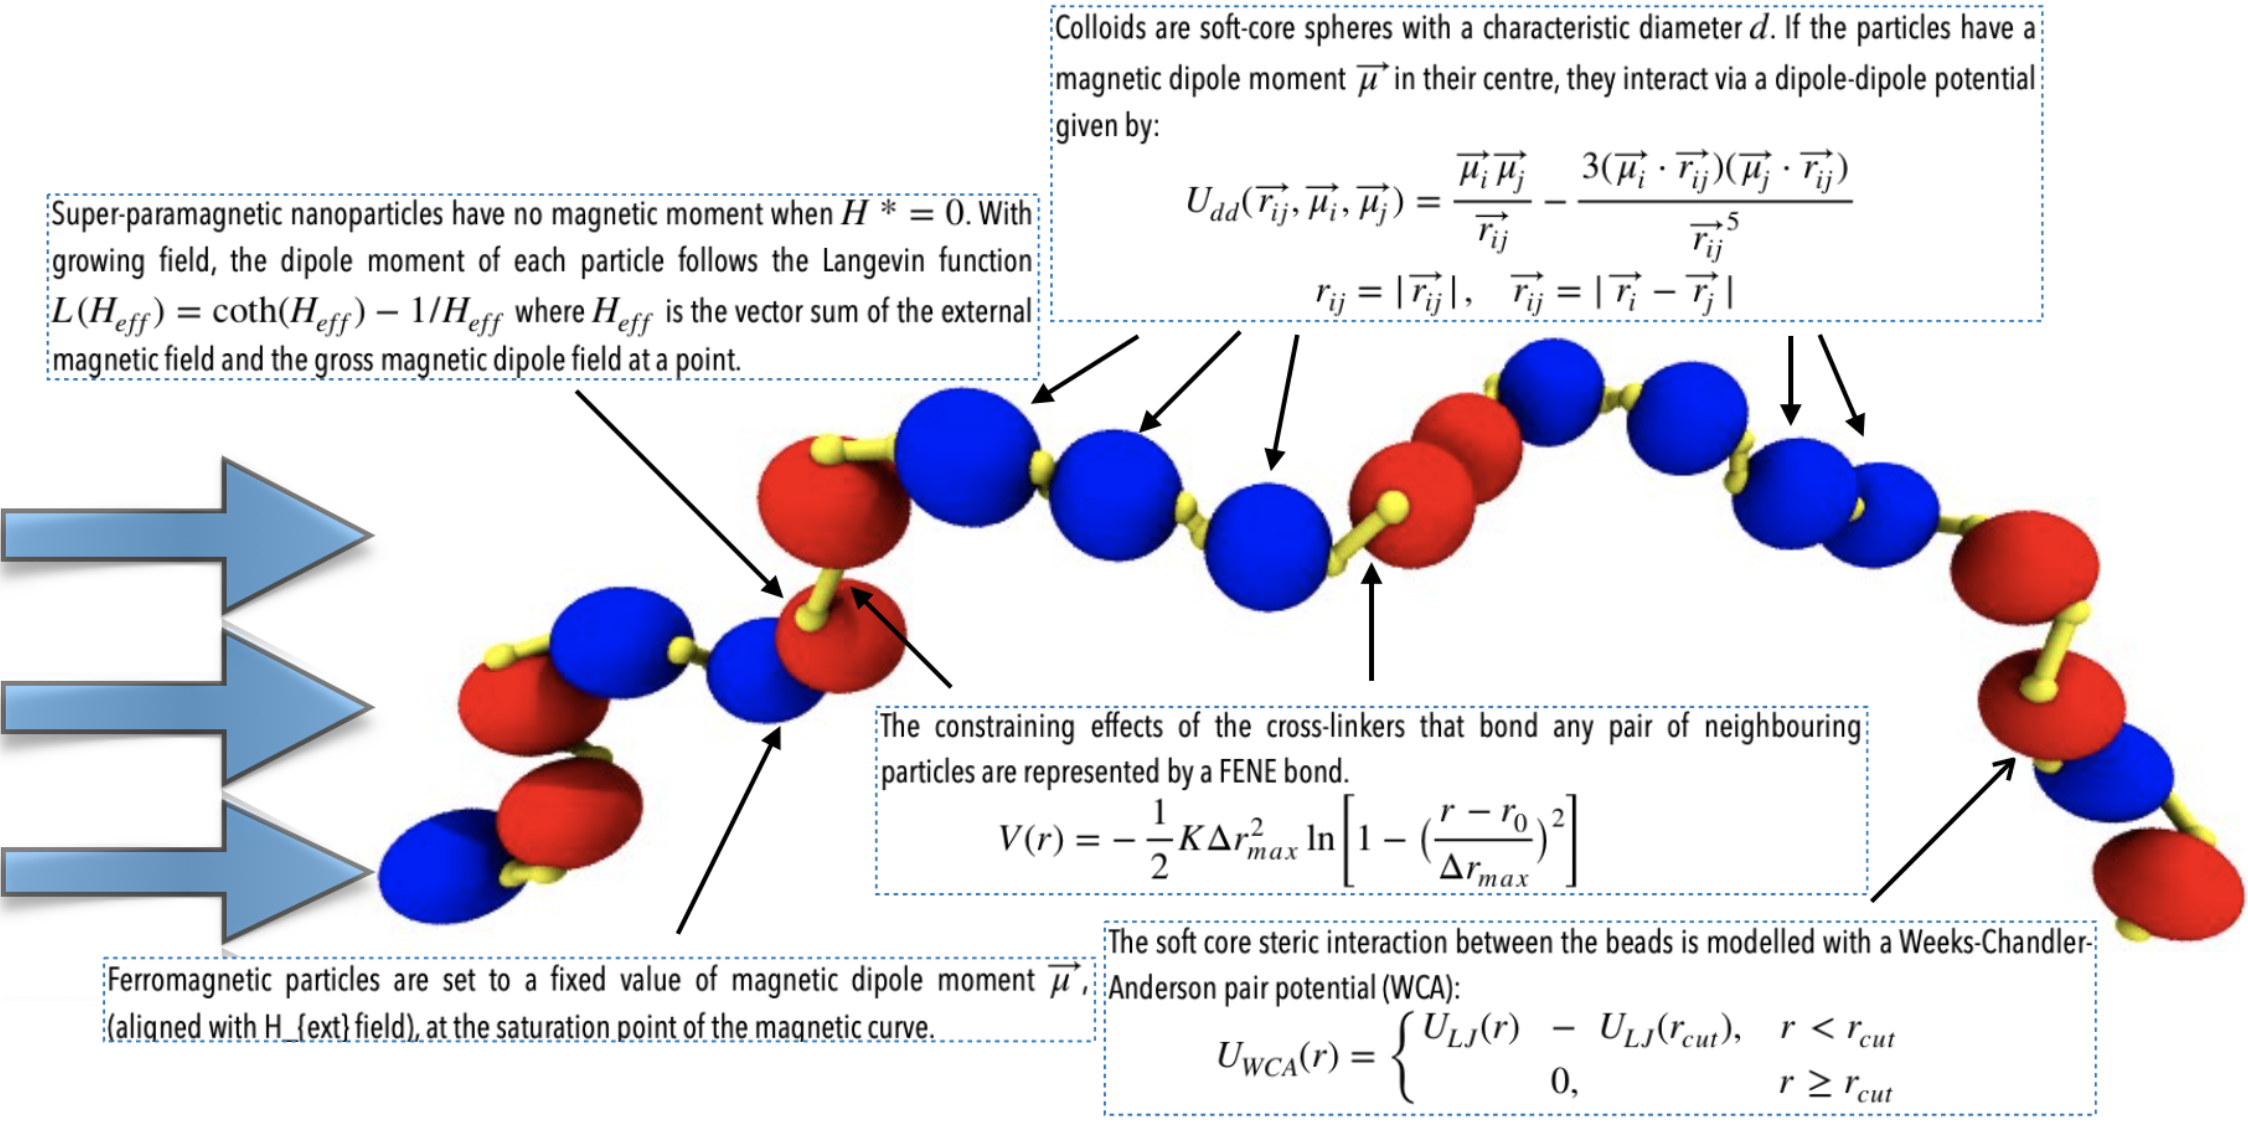
\includegraphics[height=7cm]{fig2}
\end{figure}
    \item{\textbf{\textcolor{cyan}{Tasks 4}}: Extensive Lattice-Boltzmann hydrodynamics simulations will be performed within the ESPReSso framework, along with code optimisation based on the MPI and CUDA platforms. We use the P3M algorithm for taking into account long-range magnetic forces with periodic boundary conditions.\cite{cerda2008p}}
    \item{\textbf{\textcolor{MidnightBlue}{Tasks 1-2}}: The first step of is to create octahedron cages, with a size of around 30 nm, using DNA origami technology.\cite{tian2015prescribed} Some specifically designated vertices of these cages contain several single-stranded DNA segments (ssDNA) that allow to crosslink different cages by hybridising their corresponding ssDNA. The selection of such binding vertices, that is fully controllable in experiments by means of the DNA sequence encoding,\cite{tian2015prescribed} determines the self-assembly structure of the cages. For linear chains we need binding sites placed at opposite vertices of the octahedra, Fig. 2a. Additionally, every cage will contain several ssDNA pointed towards its inner region. Therefore, a nanoparticle functionalized with complementary ssDNA that enters such a region will become cross-linked to the cage structure.\cite{sun2013dna,zhang2013general} An example of these structures as observed by TEM is shown in Fig. 2a. For filaments with ferromagnetic particles, the second step of the experimental protocol will be the placement of the MPs into the cages with a particular orientation of their magnetic dipoles with respect to the binding vertices of the octahedra. Here, we would rely on the results of the simulation to estimate the fields needed to orient the particles. Firstly, the empty cages will be immobilised on a surface previously functionalized with ssDNA complementary to the strands of one of the binding vertices,\cite{maye2009stepwise} shown in Fig 2b. This substrate will be exposed to a solution of MPs, isotropically coated with a shell of DNA, complementary to the ssDNA of the cage’s inner region. At appropriate densities of grafted cages and MPs in suspension, the occupation of the cages and subsequent hybridisation of the cage–nanoparticle complex will be obtained. If this assembly is carried out under an external magnetic field of proper intensity and perpendicular to the surface—i.e., parallel to the line that connects the two external binding vertices of the cages—the MPs will tend to keep their magnetic moments aligned with the field and, therefore, with the external binding vertices. Once the hybridisation is completed, the cross-linkers will fix the orientation of every particle and its magnetic moment with respect to the structure of the cage that is occupying. Finally, the filled cages will be released from the surface using DNA replacement reaction, which is based on the higher affinity of complementary strands with a larger number of base-pairings. Previous studies showed that this method has a high efficiency and, moreover, leaves the filled cages fully intact and ready for the consequent assembly into chains.\cite{sun2013dna,Sun_2013} The assembly of the filled cages into chain-like filaments will be carried out by hybridising the cage’s external binding sites, located at opposite vertices of the octahedra.\cite{tian2015prescribed} The results are shown in Fig. 2c, d.}
    \begin{figure}[h]
\centering
  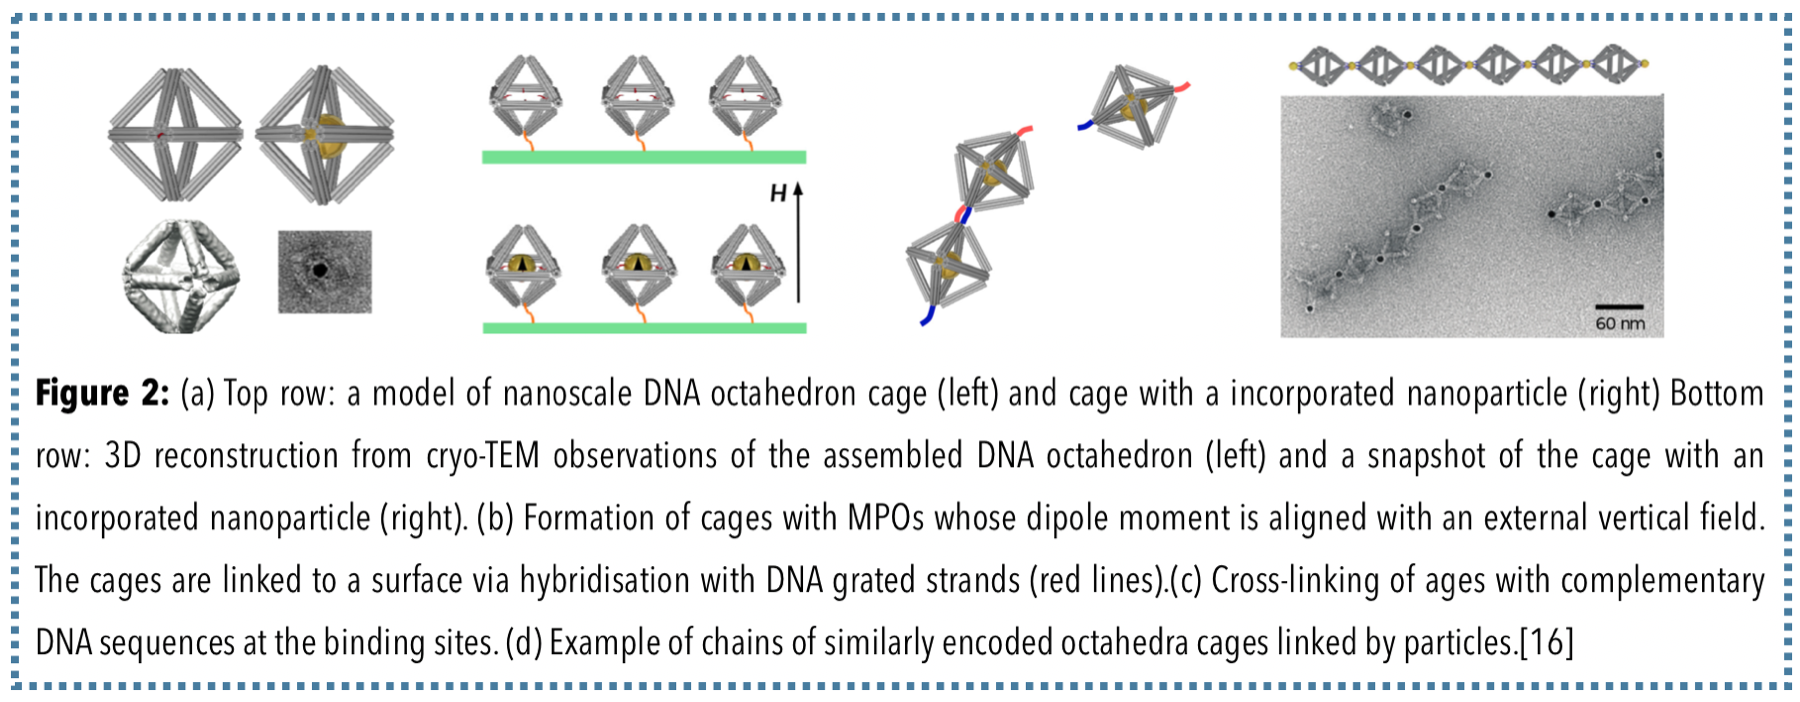
\includegraphics[height=6cm]{fig3}
\end{figure}
\end{itemize}
\subsubsection{Phase 2}
\begin{itemize}
    \item{\textbf{\textcolor{PineGreen}{Tasks 1}}: Two strategies to select the chain lengths will be tested. In the first one, the chain assembly process will be optimised to narrow the distribution of lengths down to 5 to 20 cages per filament. Then, a separation of the different length fractions will be performed by centrifugation. In the second approach, a precise control of the length will be attempted during the chain assembly by using surface stepwise growth.\cite{tian2015prescribed}}
    \item{\textbf{\textcolor{PineGreen}{Tasks 2-3}}:  visual examination of samples, global evaluation of end product. Extensive TEM, SAXS and AFM measurements and tests will be performed in efforts to precisely characterise the samples. We will attempt to achieve 1-to-1 correspondence between out computational model and the samples. We will quantify this by reproducing the behaviour of the sample in various test scenarios. }
\end{itemize}


\bibliographystyle{apacite}
\bibliography{magfils}

\end{document}